\documentclass{article}\usepackage[]{graphicx}\usepackage[]{color}
%% maxwidth is the original width if it is less than linewidth
%% otherwise use linewidth (to make sure the graphics do not exceed the margin)
\makeatletter
\def\maxwidth{ %
  \ifdim\Gin@nat@width>\linewidth
    \linewidth
  \else
    \Gin@nat@width
  \fi
}
\makeatother

\definecolor{fgcolor}{rgb}{0.345, 0.345, 0.345}
\newcommand{\hlnum}[1]{\textcolor[rgb]{0.686,0.059,0.569}{#1}}%
\newcommand{\hlstr}[1]{\textcolor[rgb]{0.192,0.494,0.8}{#1}}%
\newcommand{\hlcom}[1]{\textcolor[rgb]{0.678,0.584,0.686}{\textit{#1}}}%
\newcommand{\hlopt}[1]{\textcolor[rgb]{0,0,0}{#1}}%
\newcommand{\hlstd}[1]{\textcolor[rgb]{0.345,0.345,0.345}{#1}}%
\newcommand{\hlkwa}[1]{\textcolor[rgb]{0.161,0.373,0.58}{\textbf{#1}}}%
\newcommand{\hlkwb}[1]{\textcolor[rgb]{0.69,0.353,0.396}{#1}}%
\newcommand{\hlkwc}[1]{\textcolor[rgb]{0.333,0.667,0.333}{#1}}%
\newcommand{\hlkwd}[1]{\textcolor[rgb]{0.737,0.353,0.396}{\textbf{#1}}}%

\usepackage{framed}
\makeatletter
\newenvironment{kframe}{%
 \def\at@end@of@kframe{}%
 \ifinner\ifhmode%
  \def\at@end@of@kframe{\end{minipage}}%
  \begin{minipage}{\columnwidth}%
 \fi\fi%
 \def\FrameCommand##1{\hskip\@totalleftmargin \hskip-\fboxsep
 \colorbox{shadecolor}{##1}\hskip-\fboxsep
     % There is no \\@totalrightmargin, so:
     \hskip-\linewidth \hskip-\@totalleftmargin \hskip\columnwidth}%
 \MakeFramed {\advance\hsize-\width
   \@totalleftmargin\z@ \linewidth\hsize
   \@setminipage}}%
 {\par\unskip\endMakeFramed%
 \at@end@of@kframe}
\makeatother

\definecolor{shadecolor}{rgb}{.97, .97, .97}
\definecolor{messagecolor}{rgb}{0, 0, 0}
\definecolor{warningcolor}{rgb}{1, 0, 1}
\definecolor{errorcolor}{rgb}{1, 0, 0}
\newenvironment{knitrout}{}{} % an empty environment to be redefined in TeX

\usepackage{alltt}
\usepackage[sc]{mathpazo}
\usepackage[T1]{fontenc}
\usepackage{geometry}
\geometry{verbose,tmargin=2.5cm,bmargin=2.5cm,lmargin=2.5cm,rmargin=2.5cm}
\setcounter{secnumdepth}{2}
\setcounter{tocdepth}{2}
\usepackage{url}
\usepackage[unicode=true,pdfusetitle,
 bookmarks=true,bookmarksnumbered=true,bookmarksopen=true,bookmarksopenlevel=2,
 breaklinks=false,pdfborder={0 0 1},backref=false,colorlinks=false]
 {hyperref}
\hypersetup{
 pdfstartview={XYZ null null 1}}
\usepackage{breakurl}
\IfFileExists{upquote.sty}{\usepackage{upquote}}{}
\begin{document}



\title{Stat 154 Problem Set Two}


\author{Jinze Gu SID:24968967}


\maketitle

\section*{Problem One}

I used three types of dimension reduction method here, namely, PCA, kernel PCA and cmd scaling to reduce the dimension of data. Besides, I did different clusters after the dimension reduction. This is a classic example showing that we are able to cluster data in a better way after PCA. I suppose this is due to the fact that predictors are more correlated under the setup of problem is voting scenario. \\
Furthermore, we can do a loadings analysis, which shows us that there are mainly three types of voting results or there are three groups of voters in these 669 number of votings, namely, one group of people are against the proposal, another group is not against and the other group have no opinions. Although it is really naive result, I feel it is impressive to know that this is the trend from the perspective of data analysis. \\
\\
Comment: \\
As we can see from the model:\\
Firstly, as k increases, variance will explain less EPE while bias will explain more EPE for knn method. Expected EPE is also decreasing with increasing k.\\
\\
Secondly, linear fit and quadratic fit is no better than knn fit, which is what we should have noticed; because we know that the data is generated by an oscillating model and the limited points are not enough for us to draw a big picture of data.\\  


\begin{knitrout}
\definecolor{shadecolor}{rgb}{0.969, 0.969, 0.969}\color{fgcolor}\begin{kframe}
\begin{alltt}
\hlkwd{setwd}\hlstd{(}\hlstr{"/Volumes/有能出没/Stat 154/HW_2"}\hlstd{)}
\hlkwd{par}\hlstd{(}\hlkwc{mfcol} \hlstd{=} \hlkwd{c}\hlstd{(}\hlnum{2}\hlstd{,} \hlnum{2}\hlstd{))}
\hlstd{Vote} \hlkwb{<-} \hlkwd{read.table}\hlstd{(}\hlstr{"VotingRecord.txt"}\hlstd{)}
\hlstd{HouseRep} \hlkwb{<-} \hlkwd{read.table}\hlstd{(}\hlstr{"HouseMember.txt"}\hlstd{,} \hlkwc{sep} \hlstd{=} \hlstr{"\textbackslash{}t"}\hlstd{)}
\hlstd{Vote} \hlkwb{<-} \hlkwd{as.data.frame}\hlstd{(Vote)}
\hlcom{# PCA}
\hlstd{pc_vote} \hlkwb{<-} \hlkwd{prcomp}\hlstd{(Vote,} \hlkwc{rtex} \hlstd{=} \hlnum{TRUE}\hlstd{)}
\hlkwd{plot}\hlstd{(pc_vote}\hlopt{$}\hlstd{x[,} \hlnum{1}\hlstd{], pc_vote}\hlopt{$}\hlstd{x[,} \hlnum{2}\hlstd{],} \hlkwc{xlab} \hlstd{=} \hlstr{"First Principal Component"}\hlstd{,} \hlkwc{ylab} \hlstd{=} \hlstr{"Second Principal Component"}\hlstd{,}
    \hlkwc{main} \hlstd{=} \hlstr{"Projected Data in First/Second PC direction"}\hlstd{)}
\hlkwd{plot}\hlstd{(pc_vote}\hlopt{$}\hlstd{rotation[,} \hlnum{1}\hlstd{], pc_vote}\hlopt{$}\hlstd{rotation[,} \hlnum{2}\hlstd{],} \hlkwc{xlab} \hlstd{=} \hlstr{"First Principal Component"}\hlstd{,} \hlkwc{ylab} \hlstd{=} \hlstr{"Second Principal Component"}\hlstd{,}
    \hlkwc{main} \hlstd{=} \hlstr{"Loadings Analysis"}\hlstd{)}
\hlcom{# Now we can cluster the data based on first and second dimension}
\hlstd{cl_kmean} \hlkwb{<-} \hlkwd{kmeans}\hlstd{(}\hlkwd{cbind}\hlstd{(pc_vote}\hlopt{$}\hlstd{x[,} \hlnum{1}\hlstd{], pc_vote}\hlopt{$}\hlstd{x[,} \hlnum{2}\hlstd{]),} \hlkwc{centers} \hlstd{=} \hlnum{2}\hlstd{,} \hlkwc{nstart} \hlstd{=} \hlnum{1}\hlstd{)}
\hlkwd{plot}\hlstd{(}\hlkwd{cbind}\hlstd{(pc_vote}\hlopt{$}\hlstd{x[,} \hlnum{1}\hlstd{], pc_vote}\hlopt{$}\hlstd{x[,} \hlnum{2}\hlstd{]),} \hlkwc{col} \hlstd{= (cl_kmean}\hlopt{$}\hlstd{cluster} \hlopt{+} \hlnum{2}\hlstd{),} \hlkwc{xlab} \hlstd{=} \hlstr{"PC_1"}\hlstd{,} \hlkwc{ylab} \hlstd{=} \hlstr{"PC_2"}\hlstd{,}
    \hlkwc{main} \hlstd{=} \hlstr{"K-means Cluster"}\hlstd{)}
\hlcom{# Kernel PCA}
\hlkwd{library}\hlstd{(kernlab)}
\end{alltt}


{\ttfamily\noindent\color{warningcolor}{\#\# Warning: package 'kernlab' was built under R version 3.0.2}}\begin{alltt}
\hlstd{rbf} \hlkwb{<-} \hlkwd{rbfdot}\hlstd{(}\hlkwc{sigma} \hlstd{=} \hlnum{0.001}\hlstd{)}
\hlstd{kpcma_vote} \hlkwb{<-} \hlkwd{kernelMatrix}\hlstd{(rbf,} \hlkwd{as.matrix}\hlstd{(Vote))}
\hlstd{kpc_vote} \hlkwb{<-} \hlkwd{kpca}\hlstd{(kpcma_vote)}
\hlkwd{plot}\hlstd{(}\hlkwd{eig}\hlstd{(kpc_vote),} \hlkwc{main} \hlstd{=} \hlstr{"Kernel PCA Scree Plot"}\hlstd{,} \hlkwc{ylab} \hlstd{=} \hlstr{"EigenValue"}\hlstd{)}
\end{alltt}
\end{kframe}
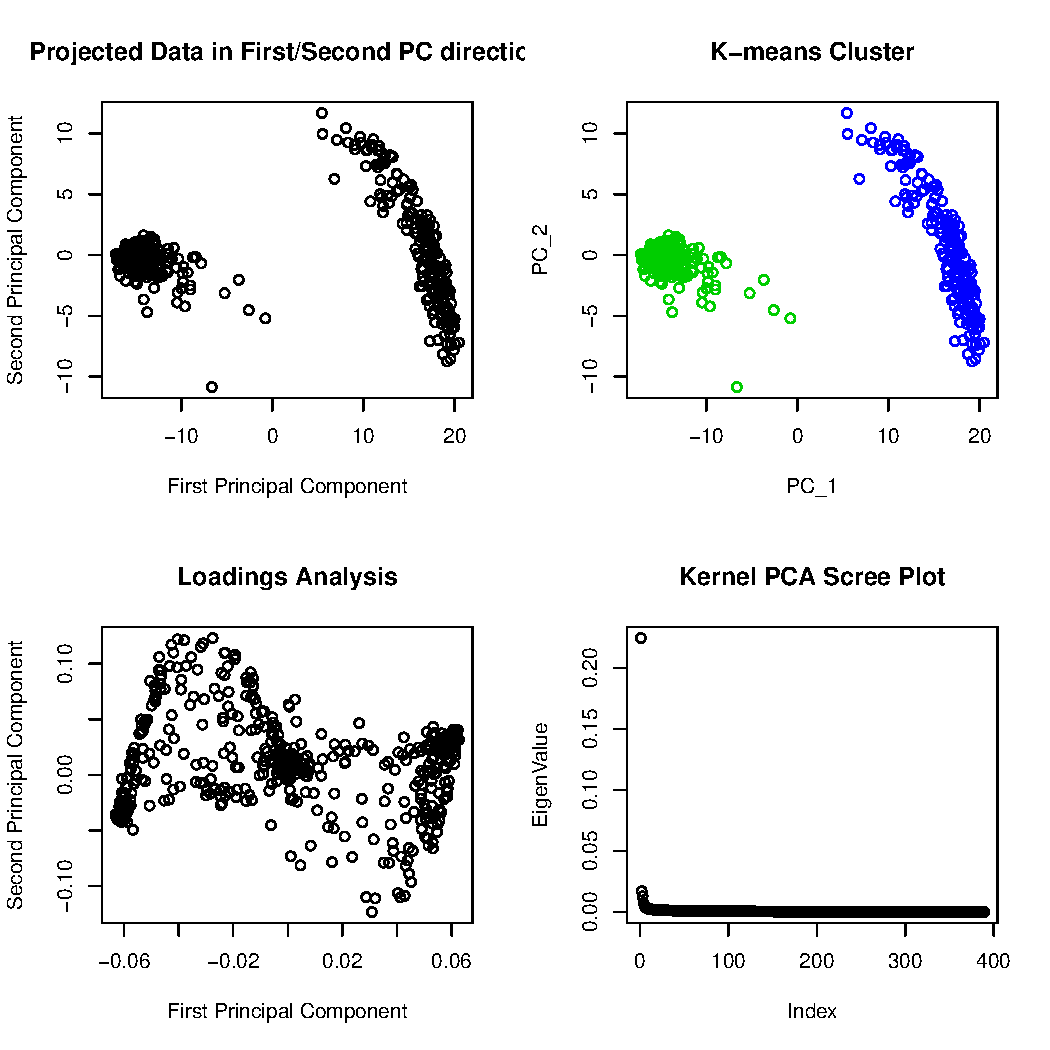
\includegraphics[width=\maxwidth]{figure/minimal-Problem_One1} 
\begin{kframe}\begin{alltt}
\hlkwd{plot}\hlstd{(}\hlkwd{rotated}\hlstd{(kpc_vote)[,} \hlnum{1}\hlstd{],} \hlkwd{rotated}\hlstd{(kpc_vote)[,} \hlnum{2}\hlstd{])}
\hlcom{## Now I will use K-medoids to cluster the data using Euclidean distance}
\hlkwd{library}\hlstd{(cluster)}
\hlstd{diss_vote_1} \hlkwb{<-} \hlkwd{dist}\hlstd{(}\hlkwd{cbind}\hlstd{(}\hlkwd{rotated}\hlstd{(kpc_vote)[,} \hlnum{1}\hlstd{],} \hlkwd{rotated}\hlstd{(kpc_vote)[,} \hlnum{2}\hlstd{]),} \hlkwc{method} \hlstd{=} \hlstr{"euclidean"}\hlstd{)}
\hlstd{kmed_vote_1} \hlkwb{<-} \hlkwd{pam}\hlstd{(diss_vote_1,} \hlkwc{k} \hlstd{=} \hlnum{2}\hlstd{)}
\hlkwd{plot}\hlstd{(}\hlkwd{cbind}\hlstd{(}\hlkwd{rotated}\hlstd{(kpc_vote)[,} \hlnum{1}\hlstd{],} \hlkwd{rotated}\hlstd{(kpc_vote)[,} \hlnum{2}\hlstd{]),} \hlkwc{col} \hlstd{= (kmed_vote_1}\hlopt{$}\hlstd{clustering} \hlopt{+}
    \hlnum{2}\hlstd{),} \hlkwc{xlab} \hlstd{=} \hlstr{""}\hlstd{,} \hlkwc{ylab} \hlstd{=} \hlstr{""}\hlstd{,} \hlkwc{main} \hlstd{=} \hlstr{"Euclidean Metric"}\hlstd{)}
\hlstd{diss_vote_2} \hlkwb{<-} \hlkwd{dist}\hlstd{(}\hlkwd{cbind}\hlstd{(}\hlkwd{rotated}\hlstd{(kpc_vote)[,} \hlnum{1}\hlstd{],} \hlkwd{rotated}\hlstd{(kpc_vote)[,} \hlnum{2}\hlstd{]),} \hlkwc{method} \hlstd{=} \hlstr{"manhattan"}\hlstd{)}
\hlstd{kmed_vote_2} \hlkwb{<-} \hlkwd{pam}\hlstd{(diss_vote_2,} \hlkwc{k} \hlstd{=} \hlnum{2}\hlstd{)}
\hlkwd{plot}\hlstd{(}\hlkwd{cbind}\hlstd{(}\hlkwd{rotated}\hlstd{(kpc_vote)[,} \hlnum{1}\hlstd{],} \hlkwd{rotated}\hlstd{(kpc_vote)[,} \hlnum{2}\hlstd{]),} \hlkwc{col} \hlstd{= (kmed_vote_2}\hlopt{$}\hlstd{clustering} \hlopt{+}
    \hlnum{2}\hlstd{),} \hlkwc{xlab} \hlstd{=} \hlstr{""}\hlstd{,} \hlkwc{ylab} \hlstd{=} \hlstr{""}\hlstd{,} \hlkwc{main} \hlstd{=} \hlstr{"Manhattan Metric"}\hlstd{)}
\hlstd{diss_vote_3} \hlkwb{<-} \hlkwd{dist}\hlstd{(}\hlkwd{cbind}\hlstd{(}\hlkwd{rotated}\hlstd{(kpc_vote)[,} \hlnum{1}\hlstd{],} \hlkwd{rotated}\hlstd{(kpc_vote)[,} \hlnum{2}\hlstd{]),} \hlkwc{method} \hlstd{=} \hlstr{"maximum"}\hlstd{)}
\hlstd{kmed_vote_3} \hlkwb{<-} \hlkwd{pam}\hlstd{(diss_vote_3,} \hlkwc{k} \hlstd{=} \hlnum{2}\hlstd{)}
\hlkwd{plot}\hlstd{(}\hlkwd{cbind}\hlstd{(}\hlkwd{rotated}\hlstd{(kpc_vote)[,} \hlnum{1}\hlstd{],} \hlkwd{rotated}\hlstd{(kpc_vote)[,} \hlnum{2}\hlstd{]),} \hlkwc{col} \hlstd{= (kmed_vote_3}\hlopt{$}\hlstd{clustering} \hlopt{+}
    \hlnum{2}\hlstd{),} \hlkwc{xlab} \hlstd{=} \hlstr{""}\hlstd{,} \hlkwc{ylab} \hlstd{=} \hlstr{""}\hlstd{,} \hlkwc{main} \hlstd{=} \hlstr{"Maximum Metric"}\hlstd{)}
\end{alltt}
\end{kframe}
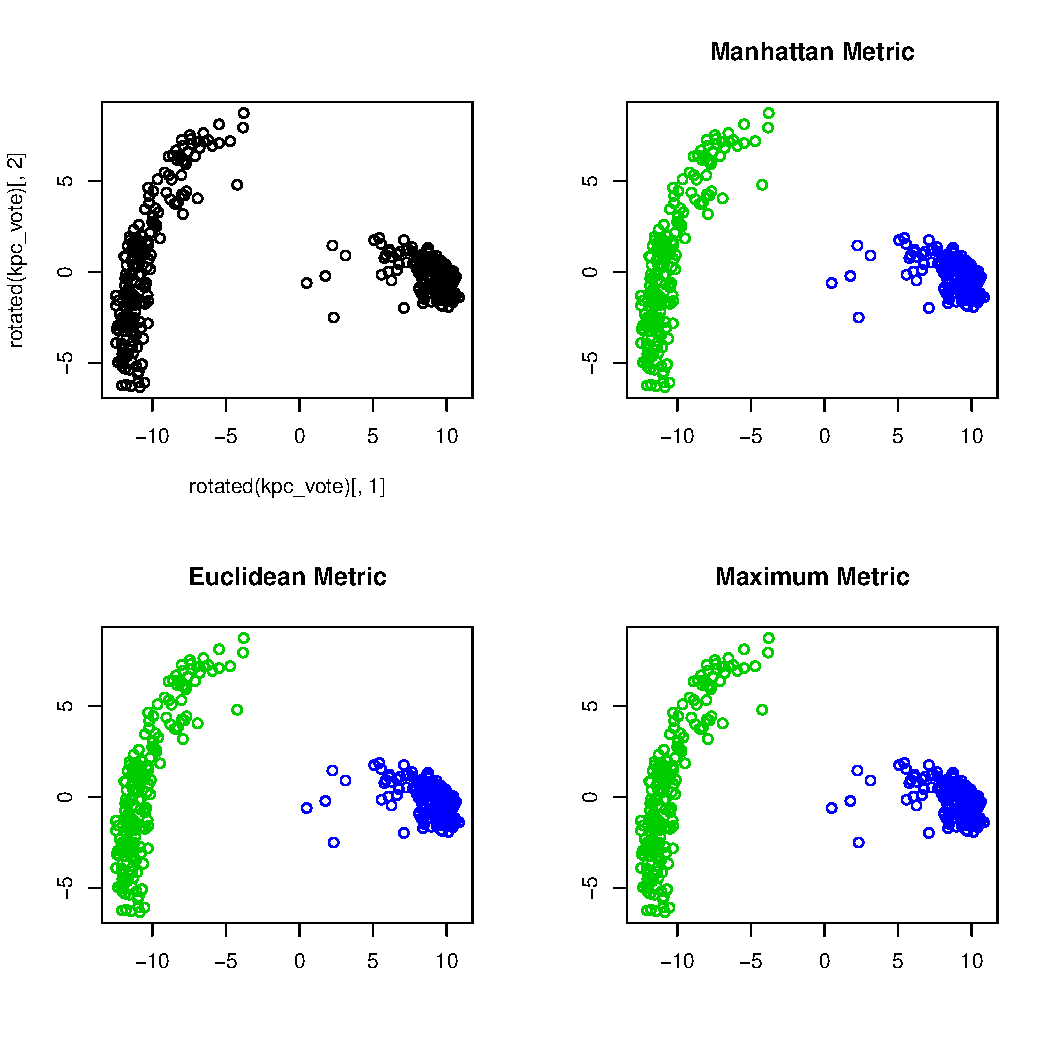
\includegraphics[width=\maxwidth]{figure/minimal-Problem_One2} 
\begin{kframe}\begin{alltt}
\hlcom{## After kernel PCA, we can do a H-cluster}
\hlstd{dis_euc} \hlkwb{<-} \hlkwd{hclust}\hlstd{(diss_vote_1,} \hlkwc{method} \hlstd{=} \hlstr{"complete"}\hlstd{)}
\hlkwd{plclust}\hlstd{(dis_euc,} \hlkwc{labels} \hlstd{=} \hlnum{FALSE}\hlstd{,} \hlkwc{main} \hlstd{=} \hlstr{"Complete Metric H-cluster"}\hlstd{)}
\hlstd{dis_man} \hlkwb{<-} \hlkwd{hclust}\hlstd{(diss_vote_2,} \hlkwc{method} \hlstd{=} \hlstr{"single"}\hlstd{)}
\hlkwd{plclust}\hlstd{(dis_man,} \hlkwc{labels} \hlstd{=} \hlnum{FALSE}\hlstd{, ,} \hlkwc{main} \hlstd{=} \hlstr{"Single Metric H-cluster"}\hlstd{)}
\hlstd{dis_max} \hlkwb{<-} \hlkwd{hclust}\hlstd{(diss_vote_3,} \hlkwc{method} \hlstd{=} \hlstr{"average"}\hlstd{)}
\hlkwd{plclust}\hlstd{(dis_max,} \hlkwc{labels} \hlstd{=} \hlnum{FALSE}\hlstd{, ,} \hlkwc{main} \hlstd{=} \hlstr{"Average Metric H-cluster"}\hlstd{)}
\hlcom{# Using CMDscale}
\hlkwd{par}\hlstd{(}\hlkwc{mfcol} \hlstd{=} \hlkwd{c}\hlstd{(}\hlnum{2}\hlstd{,} \hlnum{1}\hlstd{))}
\hlkwd{plot}\hlstd{(}\hlkwd{cmdscale}\hlstd{(}\hlkwd{dist}\hlstd{(Vote),} \hlkwc{k} \hlstd{=} \hlnum{2}\hlstd{),} \hlkwc{main} \hlstd{=} \hlstr{" CMD scale using Euclidean Metric"}\hlstd{,} \hlkwc{xlab} \hlstd{=} \hlstr{"CMD PC One"}\hlstd{,}
    \hlkwc{ylab} \hlstd{=} \hlstr{"CMD PC TWO"}\hlstd{)}
\hlkwd{plot}\hlstd{(}\hlkwd{cmdscale}\hlstd{(}\hlkwd{dist}\hlstd{(Vote,} \hlkwc{method} \hlstd{=} \hlstr{"manhattan"}\hlstd{),} \hlkwc{k} \hlstd{=} \hlnum{2}\hlstd{),} \hlkwc{main} \hlstd{=} \hlstr{" CMD scale using Manhattan Metric"}\hlstd{,}
    \hlkwc{xlab} \hlstd{=} \hlstr{"CMD PC One"}\hlstd{,} \hlkwc{ylab} \hlstd{=} \hlstr{"CMD PC Two"}\hlstd{)}
\end{alltt}
\end{kframe}
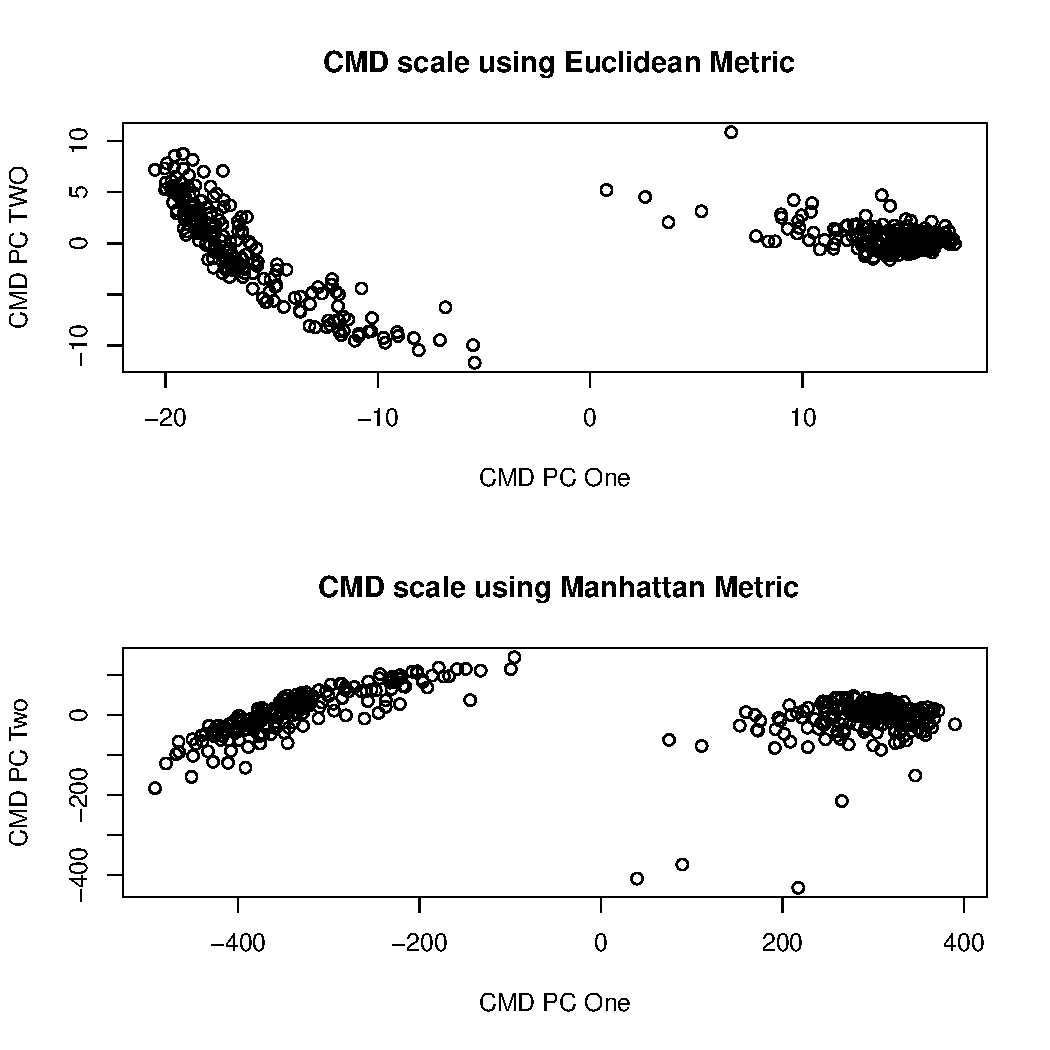
\includegraphics[width=\maxwidth]{figure/minimal-Problem_One3} 

\end{knitrout}


\section*{Problem Two}
\begin{knitrout}
\definecolor{shadecolor}{rgb}{0.969, 0.969, 0.969}\color{fgcolor}\begin{kframe}
\begin{alltt}
\hlkwd{set.seed}\hlstd{(}\hlnum{25041}\hlstd{)}
\hlkwd{par}\hlstd{(}\hlkwc{mfcol} \hlstd{=} \hlkwd{c}\hlstd{(}\hlnum{2}\hlstd{,} \hlnum{2}\hlstd{))}
\hlkwd{require}\hlstd{(FNN)}
\end{alltt}


{\ttfamily\noindent\itshape\color{messagecolor}{\#\# Loading required package: FNN}}

{\ttfamily\noindent\color{warningcolor}{\#\# Warning: package 'FNN' was built under R version 3.0.2}}\begin{alltt}
\hlkwd{require}\hlstd{(fields)}
\end{alltt}


{\ttfamily\noindent\itshape\color{messagecolor}{\#\# Loading required package: fields\\\#\# Loading required package: spam\\\#\# Loading required package: grid\\\#\# Spam version 0.40-0 (2013-09-11) is loaded.\\\#\# Type 'help( Spam)' or 'demo( spam)' for a short introduction \\\#\# and overview of this package.\\\#\# Help for individual functions is also obtained by adding the\\\#\# suffix '.spam' to the function name, e.g. 'help( chol.spam)'.\\\#\# \\\#\# Attaching package: 'spam'\\\#\# \\\#\# 下列对象被屏蔽了from 'package:base':\\\#\# \\\#\#\ \ \ \  backsolve, forwardsolve\\\#\# \\\#\# Loading required package: maps}}\begin{alltt}
\hlstd{X} \hlkwb{<-} \hlstd{(}\hlkwd{c}\hlstd{(}\hlnum{1}\hlopt{:}\hlnum{10}\hlstd{)} \hlopt{-} \hlnum{1}\hlopt{/}\hlnum{2}\hlstd{)}\hlopt{/}\hlnum{10} \hlopt{*} \hlnum{2} \hlopt{*} \hlstd{pi}
\hlstd{Y} \hlkwb{<-} \hlkwd{cos}\hlstd{(}\hlnum{10} \hlopt{*} \hlstd{X)} \hlopt{+} \hlnum{2} \hlopt{+} \hlkwd{rnorm}\hlstd{(}\hlnum{10}\hlstd{,} \hlkwc{sd} \hlstd{=} \hlkwd{sqrt}\hlstd{(}\hlnum{0.1}\hlstd{))}
\hlcom{# 1) # This is the k-nn funtion that returns the estimated value of some point using k}
\hlcom{# nearest neighbors with Euclidean metric}
\hlstd{knn} \hlkwb{<-} \hlkwa{function}\hlstd{(}\hlkwc{x}\hlstd{,} \hlkwc{y}\hlstd{,} \hlkwc{xseq}\hlstd{,} \hlkwc{k}\hlstd{) \{}
    \hlkwa{if} \hlstd{(k} \hlopt{<} \hlkwd{length}\hlstd{(x)) \{}
        \hlstd{dmat} \hlkwb{<-} \hlkwd{rdist}\hlstd{(x, xseq)}
        \hlstd{indices} \hlkwb{<-} \hlkwd{order}\hlstd{(dmat)[}\hlnum{2}\hlopt{:}\hlstd{(k} \hlopt{+} \hlnum{1}\hlstd{)]}  \hlcom{# If you need to find less than 10 neighbors, it will not take the point itself as a neighbor}
        \hlkwd{return}\hlstd{(}\hlkwd{mean}\hlstd{(y[indices]))}
    \hlstd{\}} \hlkwa{else} \hlstd{\{}
        \hlstd{dmat} \hlkwb{<-} \hlkwd{rdist}\hlstd{(x, xseq)}
        \hlstd{indices} \hlkwb{<-} \hlkwd{order}\hlstd{(dmat)[}\hlnum{1}\hlopt{:}\hlstd{k]}
        \hlcom{# If you need to find 10 neighbors, it will take the points itself as a neighbor}
        \hlkwd{return}\hlstd{(}\hlkwd{mean}\hlstd{(y[indices]))}
    \hlstd{\}}
\hlstd{\}}
\hlcom{# Plot knn function for k = 1,3,10}
\hlstd{knn_one} \hlkwb{<-} \hlkwd{sapply}\hlstd{(X, knn,} \hlkwc{y} \hlstd{= Y,} \hlkwc{xseq} \hlstd{= X,} \hlkwc{k} \hlstd{=} \hlnum{1}\hlstd{)}
\hlkwd{plot}\hlstd{(X, Y,} \hlkwc{main} \hlstd{=} \hlstr{"k-nearest-neighbor k = 1"}\hlstd{)}
\hlkwd{points}\hlstd{(X, knn_one,} \hlkwc{pch} \hlstd{=} \hlnum{4}\hlstd{)}
\hlkwd{legend}\hlstd{(}\hlstr{"bottomleft"}\hlstd{,} \hlkwd{c}\hlstd{(}\hlstr{"original points"}\hlstd{,} \hlstr{"fitted points"}\hlstd{),} \hlkwc{pch} \hlstd{=} \hlkwd{c}\hlstd{(}\hlnum{1}\hlstd{,} \hlnum{4}\hlstd{))}
\hlstd{knn_thr} \hlkwb{<-} \hlkwd{sapply}\hlstd{(X, knn,} \hlkwc{y} \hlstd{= Y,} \hlkwc{xseq} \hlstd{= X,} \hlkwc{k} \hlstd{=} \hlnum{3}\hlstd{)}
\hlkwd{plot}\hlstd{(X, Y,} \hlkwc{main} \hlstd{=} \hlstr{"k-nearest-neighbor k = 3"}\hlstd{)}
\hlkwd{points}\hlstd{(X, knn_thr,} \hlkwc{pch} \hlstd{=} \hlnum{4}\hlstd{)}
\hlkwd{legend}\hlstd{(}\hlstr{"bottomleft"}\hlstd{,} \hlkwd{c}\hlstd{(}\hlstr{"original points"}\hlstd{,} \hlstr{"fitted points"}\hlstd{),} \hlkwc{pch} \hlstd{=} \hlkwd{c}\hlstd{(}\hlnum{1}\hlstd{,} \hlnum{4}\hlstd{))}
\hlstd{knn_ten} \hlkwb{<-} \hlkwd{sapply}\hlstd{(X, knn,} \hlkwc{y} \hlstd{= Y,} \hlkwc{xseq} \hlstd{= X,} \hlkwc{k} \hlstd{=} \hlnum{10}\hlstd{)}
\hlkwd{plot}\hlstd{(X, Y,} \hlkwc{main} \hlstd{=} \hlstr{"k-nearest-neighbor k = 10"}\hlstd{)}
\hlkwd{points}\hlstd{(X, knn_ten,} \hlkwc{pch} \hlstd{=} \hlnum{4}\hlstd{)}
\hlkwd{legend}\hlstd{(}\hlstr{"bottomleft"}\hlstd{,} \hlkwd{c}\hlstd{(}\hlstr{"original points"}\hlstd{,} \hlstr{"fitted points"}\hlstd{),} \hlkwc{pch} \hlstd{=} \hlkwd{c}\hlstd{(}\hlnum{1}\hlstd{,} \hlnum{4}\hlstd{))}
\hlcom{# EPE(pi) and E(EPE(X)) For each fixed X(notation is pi in problem), I decided to generate}
\hlcom{# its response 100 times(with different errors) and calculate EPE(pi). Then I conduct the}
\hlcom{# same procedure for 500 values randomly generated from UNIF(0, 2*pi) and calculate the}
\hlcom{# E(EPE(X)). In order to reduce the error effect, I use the same error 500 times for}
\hlcom{# different fixed X.}
\hlkwd{set.seed}\hlstd{(}\hlnum{12345}\hlstd{)}
\hlstd{Eps} \hlkwb{<-} \hlkwd{matrix}\hlstd{(}\hlkwd{rep}\hlstd{(}\hlkwd{rnorm}\hlstd{(}\hlnum{100}\hlstd{,} \hlkwc{sd} \hlstd{=} \hlkwd{sqrt}\hlstd{(}\hlnum{0.1}\hlstd{)),} \hlnum{500}\hlstd{),} \hlkwc{ncol} \hlstd{=} \hlnum{500}\hlstd{)}  \hlcom{# Firstly I generate random}
\hlstd{X_pre} \hlkwb{<-} \hlstd{(}\hlkwd{c}\hlstd{(}\hlnum{1}\hlopt{:}\hlnum{500}\hlstd{)} \hlopt{-} \hlnum{1}\hlopt{/}\hlnum{2}\hlstd{)}\hlopt{/}\hlnum{500} \hlopt{*} \hlnum{2} \hlopt{*} \hlstd{pi}  \hlcom{# The 500 randomly generated number from        UNIF(0, 2*pi)}
\hlstd{Simu_Y} \hlkwb{<-} \hlkwd{t}\hlstd{(}\hlkwd{matrix}\hlstd{(}\hlnum{1}\hlstd{,} \hlkwc{nrow} \hlstd{=} \hlnum{500}\hlstd{,} \hlkwc{ncol} \hlstd{=} \hlnum{100}\hlstd{)} \hlopt{*} \hlstd{(}\hlkwd{cos}\hlstd{(}\hlnum{10} \hlopt{*} \hlstd{X_pre)} \hlopt{+} \hlnum{2}\hlstd{))} \hlopt{+} \hlstd{Eps}
\hlcom{# This is the model used to fit a prediction data(data_X) with original model constructed}
\hlcom{# by Y and X, I use}
\hlstd{knn_model} \hlkwb{<-} \hlkwa{function}\hlstd{(}\hlkwc{data_X}\hlstd{,} \hlkwc{X}\hlstd{,} \hlkwc{Y}\hlstd{,} \hlkwc{k}\hlstd{) \{}
    \hlstd{fit} \hlkwb{<-} \hlkwd{sapply}\hlstd{(data_X, knn,} \hlkwc{y} \hlstd{= Y,} \hlkwc{xseq} \hlstd{= X,} \hlkwc{k} \hlstd{= k)}
    \hlstd{EPE} \hlkwb{<-} \hlkwd{matrix}\hlstd{(}\hlnum{NA}\hlstd{,} \hlkwc{nrow} \hlstd{=} \hlkwd{length}\hlstd{(data_X),} \hlkwc{ncol} \hlstd{=} \hlnum{3}\hlstd{)}
    \hlkwa{for} \hlstd{(i} \hlkwa{in} \hlnum{1}\hlopt{:}\hlkwd{length}\hlstd{(data_X)) \{}
        \hlstd{EPE[i,} \hlnum{1}\hlstd{]} \hlkwb{<-} \hlkwd{mean}\hlstd{((Simu_Y[, i]} \hlopt{-} \hlstd{fit[i])}\hlopt{^}\hlnum{2}\hlstd{)}
        \hlstd{EPE[i,} \hlnum{2}\hlstd{]} \hlkwb{<-} \hlkwd{mean}\hlstd{((Simu_Y[, i]} \hlopt{-} \hlkwd{mean}\hlstd{(Simu_Y[, i]))}\hlopt{^}\hlnum{2}\hlstd{)}
        \hlstd{EPE[i,} \hlnum{3}\hlstd{]} \hlkwb{<-} \hlkwd{mean}\hlstd{((fit[i]} \hlopt{-} \hlkwd{mean}\hlstd{(Simu_Y[, i]))}\hlopt{^}\hlnum{2}\hlstd{)}
    \hlstd{\}}
    \hlcom{# Since X's are draw from uniform distribution, so we can estimate the Expected EPE by}
    \hlcom{# taking the average of 500 different EPE}
    \hlstd{MeanEPE} \hlkwb{<-} \hlkwd{mean}\hlstd{(EPE)}\hlopt{/}\hlstd{(}\hlnum{2} \hlopt{*} \hlstd{pi)}
    \hlstd{var_ratio} \hlkwb{<-} \hlkwd{mean}\hlstd{(EPE[,} \hlnum{2}\hlstd{]}\hlopt{/}\hlstd{EPE[,} \hlnum{1}\hlstd{])}
    \hlstd{bias_ratio} \hlkwb{<-} \hlkwd{mean}\hlstd{(EPE[,} \hlnum{3}\hlstd{]}\hlopt{/}\hlstd{EPE[,} \hlnum{1}\hlstd{])}
    \hlkwd{return}\hlstd{(}\hlkwd{data.frame}\hlstd{(}\hlkwc{Mean_EPE} \hlstd{= MeanEPE,} \hlkwc{var_ratio} \hlstd{= var_ratio,} \hlkwc{bias_ratio} \hlstd{= bias_ratio))}
\hlstd{\}}
\hlkwd{knn_model}\hlstd{(X_pre, X, Y,} \hlnum{1}\hlstd{)}
\end{alltt}
\begin{verbatim}
##   Mean_EPE var_ratio bias_ratio
## 1   0.1712    0.2936     0.7064
\end{verbatim}
\begin{alltt}
\hlkwd{knn_model}\hlstd{(X_pre, X, Y,} \hlnum{3}\hlstd{)}
\end{alltt}
\begin{verbatim}
##   Mean_EPE var_ratio bias_ratio
## 1   0.1652    0.3228     0.6772
\end{verbatim}
\begin{alltt}
\hlkwd{knn_model}\hlstd{(X_pre, X, Y,} \hlnum{10}\hlstd{)}
\end{alltt}
\begin{verbatim}
##   Mean_EPE var_ratio bias_ratio
## 1   0.1635    0.3363     0.6637
\end{verbatim}
\begin{alltt}
\hlkwd{plot}\hlstd{(}\hlkwd{rbind}\hlstd{(}\hlkwd{knn_model}\hlstd{(X_pre, X, Y,} \hlnum{1}\hlstd{)}\hlopt{$}\hlstd{bias_ratio,} \hlkwd{knn_model}\hlstd{(X_pre, X, Y,} \hlnum{3}\hlstd{)}\hlopt{$}\hlstd{bias_ratio,} \hlkwd{knn_model}\hlstd{(X_pre,}
    \hlstd{X, Y,} \hlnum{10}\hlstd{)}\hlopt{$}\hlstd{bias_ratio),} \hlkwc{type} \hlstd{=} \hlstr{"b"}\hlstd{,} \hlkwc{ylim} \hlstd{=} \hlkwd{c}\hlstd{(}\hlnum{0}\hlstd{,} \hlnum{1}\hlstd{),} \hlkwc{ylab} \hlstd{=} \hlstr{""}\hlstd{,} \hlkwc{main} \hlstd{=} \hlstr{"Variance and Bias Ratio Behaviour"}\hlstd{)}
\hlkwd{lines}\hlstd{(}\hlkwd{rbind}\hlstd{(}\hlkwd{knn_model}\hlstd{(X_pre, X, Y,} \hlnum{1}\hlstd{)}\hlopt{$}\hlstd{var_ratio,} \hlkwd{knn_model}\hlstd{(X_pre, X, Y,} \hlnum{3}\hlstd{)}\hlopt{$}\hlstd{var_ratio,} \hlkwd{knn_model}\hlstd{(X_pre,}
    \hlstd{X, Y,} \hlnum{10}\hlstd{)}\hlopt{$}\hlstd{var_ratio),} \hlkwc{lty} \hlstd{=} \hlnum{4}\hlstd{)}
\hlkwd{legend}\hlstd{(}\hlstr{"topright"}\hlstd{,} \hlkwd{c}\hlstd{(}\hlstr{"bias_ratio"}\hlstd{,} \hlstr{"var_ratio"}\hlstd{),} \hlkwc{lty} \hlstd{=} \hlkwd{c}\hlstd{(}\hlnum{1}\hlstd{,} \hlnum{4}\hlstd{))}
\end{alltt}
\end{kframe}
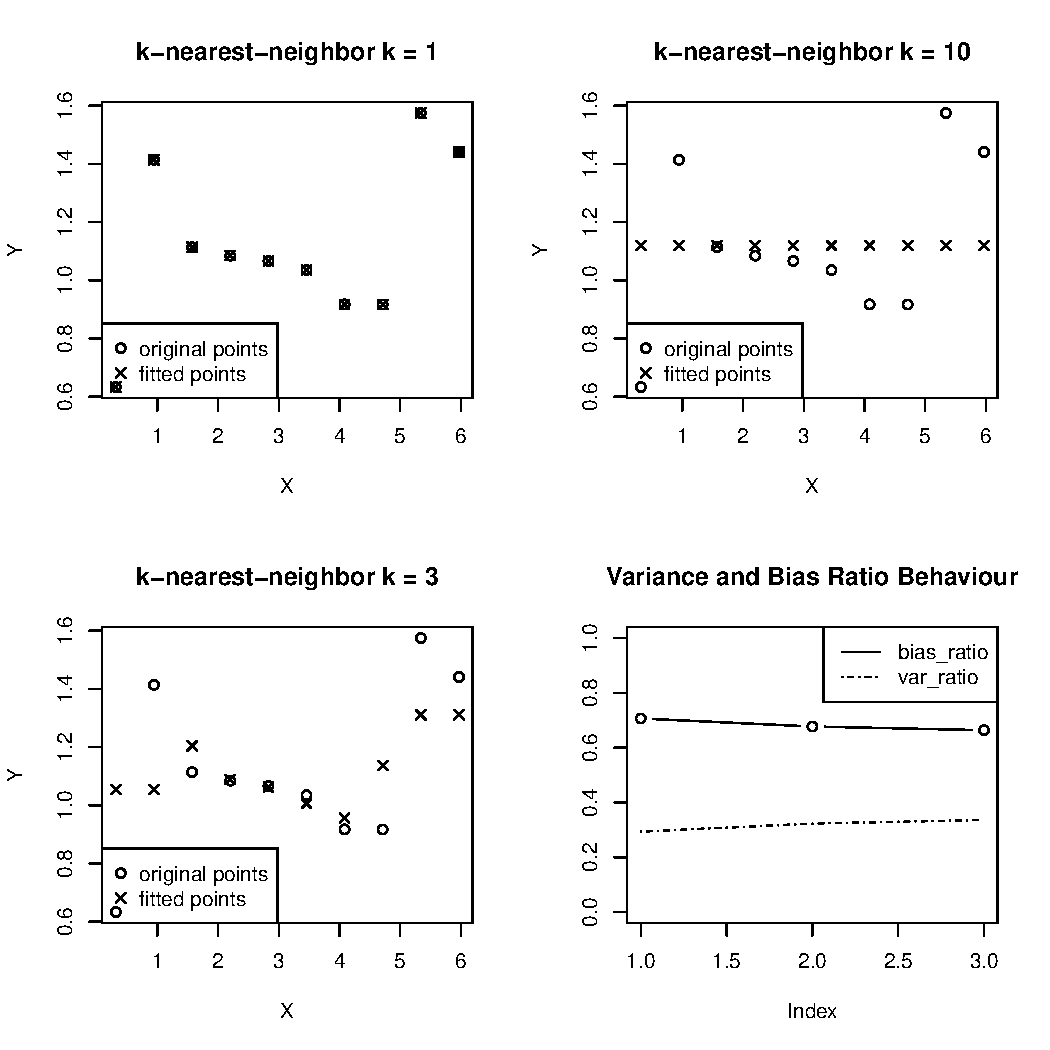
\includegraphics[width=\maxwidth]{figure/minimal-Problem_Two_One} 
\begin{kframe}\begin{alltt}
\hlcom{# Comment: It is obvious that as k increases, variance accounts for less and less in the}
\hlcom{# Expected Prediction Error and bias accounts for more and more in EPE.}
\hlcom{# Fit a constant function(The same as fitting a knn with k = 10 since we only have ten}
\hlcom{# points in the trainning sample)}
\hlkwd{knn_model}\hlstd{(X_pre, X, Y,} \hlnum{10}\hlstd{)}
\end{alltt}
\begin{verbatim}
##   Mean_EPE var_ratio bias_ratio
## 1   0.1635    0.3363     0.6637
\end{verbatim}
\begin{alltt}
\hlcom{# Comment: For constant fit, it is equivalent to fit a knn model with 10 points.}
\hlcom{# Fit a linear model}
\hlstd{fit_linear} \hlkwb{<-} \hlkwd{lm}\hlstd{(Y} \hlopt{~} \hlstd{X)}
\hlstd{predict_linear} \hlkwb{<-} \hlstd{X_pre} \hlopt{*} \hlstd{fit_linear}\hlopt{$}\hlstd{coefficients[}\hlnum{2}\hlstd{]} \hlopt{+} \hlstd{fit_linear}\hlopt{$}\hlstd{coefficients[}\hlnum{1}\hlstd{]}
\hlstd{EPE_linear} \hlkwb{<-} \hlkwd{matrix}\hlstd{(}\hlnum{NA}\hlstd{,} \hlnum{500}\hlstd{)}
\hlkwa{for} \hlstd{(i} \hlkwa{in} \hlnum{1}\hlopt{:}\hlnum{500}\hlstd{) \{}
    \hlstd{EPE_linear[i]} \hlkwb{<-} \hlkwd{mean}\hlstd{((predict_linear[i]} \hlopt{-} \hlstd{Simu_Y[, i])}\hlopt{^}\hlnum{2}\hlstd{)}
\hlstd{\}}
\hlkwd{mean}\hlstd{(EPE_linear)}\hlopt{/}\hlstd{(}\hlnum{2} \hlopt{*} \hlstd{pi)}  \hlcom{# This is the estimated E(EPE(X)) under linear model}
\end{alltt}
\begin{verbatim}
## [1] 0.2475
\end{verbatim}
\begin{alltt}
\hlstd{Var_linear} \hlkwb{<-} \hlkwd{sum}\hlstd{((}\hlkwd{mean}\hlstd{(predict_linear)} \hlopt{-} \hlstd{predict_linear)}\hlopt{^}\hlnum{2}\hlstd{)}
\hlstd{Bias_linear} \hlkwb{<-} \hlkwd{sum}\hlstd{((Simu_Y[}\hlnum{1}\hlstd{, ]} \hlopt{-} \hlkwd{mean}\hlstd{(predict_linear))}\hlopt{^}\hlnum{2}\hlstd{)}
\hlstd{Var_linear}
\end{alltt}
\begin{verbatim}
## [1] 7.238
\end{verbatim}
\begin{alltt}
\hlstd{Bias_linear}
\end{alltt}
\begin{verbatim}
## [1] 817.8
\end{verbatim}
\begin{alltt}
\hlcom{# Fit a quadratic function}
\hlstd{fit_quadra} \hlkwb{<-} \hlkwd{lm}\hlstd{(Y} \hlopt{~} \hlstd{X} \hlopt{+} \hlkwd{I}\hlstd{(X}\hlopt{^}\hlnum{2}\hlstd{))}
\hlstd{predict_quadra} \hlkwb{<-} \hlstd{X_pre}\hlopt{^}\hlnum{2} \hlopt{*} \hlstd{fit_quadra}\hlopt{$}\hlstd{coefficients[}\hlnum{3}\hlstd{]} \hlopt{+} \hlstd{X_pre} \hlopt{*} \hlstd{fit_quadra}\hlopt{$}\hlstd{coefficients[}\hlnum{2}\hlstd{]} \hlopt{+}
    \hlstd{fit_quadra}\hlopt{$}\hlstd{coefficients[}\hlnum{1}\hlstd{]}
\hlstd{EPE_quadra} \hlkwb{<-} \hlkwd{matrix}\hlstd{(}\hlnum{NA}\hlstd{,} \hlnum{500}\hlstd{)}
\hlkwa{for} \hlstd{(i} \hlkwa{in} \hlnum{1}\hlopt{:}\hlnum{500}\hlstd{) \{}
    \hlstd{EPE_quadra[i]} \hlkwb{<-} \hlkwd{mean}\hlstd{((predict_quadra[i]} \hlopt{-} \hlstd{Simu_Y[, i])}\hlopt{^}\hlnum{2}\hlstd{)}
\hlstd{\}}
\hlkwd{mean}\hlstd{(EPE_quadra)}  \hlcom{# This is the estimated E(EPE(X)) under quadratic model}
\end{alltt}
\begin{verbatim}
## [1] 1.556
\end{verbatim}
\begin{alltt}
\hlstd{Var_quadra} \hlkwb{<-} \hlkwd{sum}\hlstd{((}\hlkwd{mean}\hlstd{(predict_quadra)} \hlopt{-} \hlstd{predict_quadra)}\hlopt{^}\hlnum{2}\hlstd{)}
\hlstd{Var_quadra}
\end{alltt}
\begin{verbatim}
## [1] 8.798
\end{verbatim}
\begin{alltt}
\hlstd{Bias_quadra}
\end{alltt}


{\ttfamily\noindent\bfseries\color{errorcolor}{\#\# Error: 找不到对象'Bias\_quadra'}}\end{kframe}
\end{knitrout}



\end{document}
